% Copyright 2020 Glen Newton
% License: Creative Commons Attribution-ShareAlike 4.0 International License https://creativecommons.org/licenses/by-sa/4.0/legalcode

\documentclass[12pt]{article}
\usepackage{tikz}
\usepackage[extreme]{savetrees}
\usepackage{microtype}
\usepackage[hidelinks]{hyperref}
\usetikzlibrary{mindmap,positioning}

% from: https://tex.stackexchange.com/questions/250150/formatting-mindmap-in-tikz

\begin{document}
\sffamily
\pagestyle{empty}
          {\centering
            \makebox[0pt]{%
              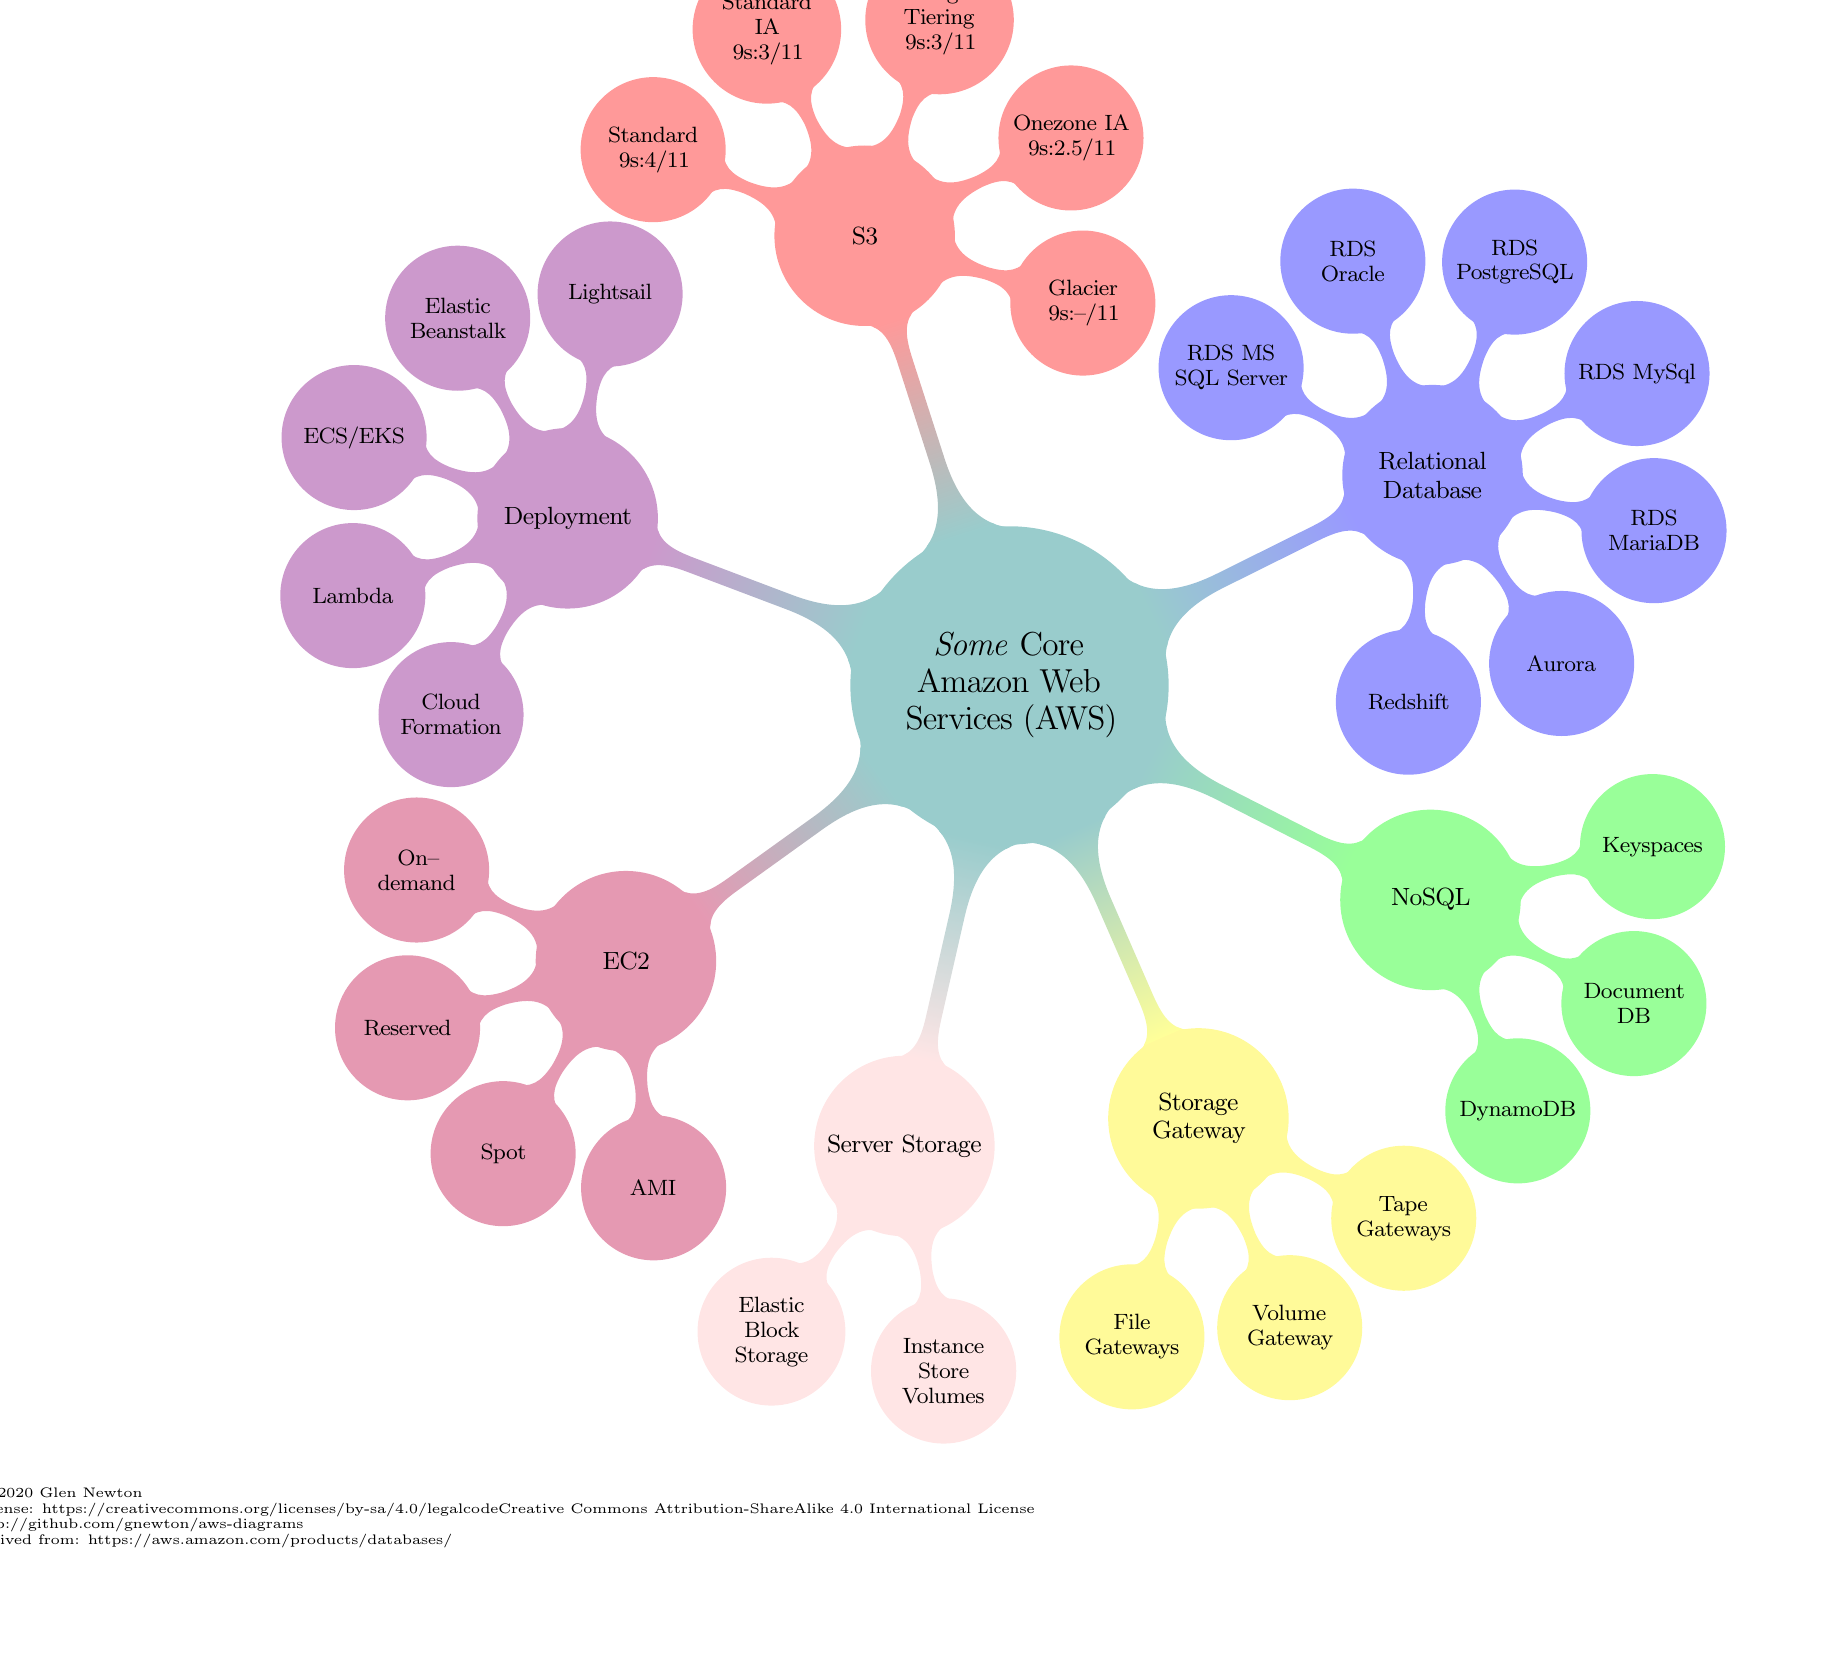
\begin{tikzpicture}
                \begin{scope}
                  [mindmap,
                    grow cyclic,
                    every node/.style=concept,
                    concept color=teal!40,
                    level 1/.append style={sibling angle=360/7, level distance=6cm},
                    level 2/.append style={sibling angle=37.5,minimum size=1.8cm},
                  ]
                  \node [root concept] {\textit{Some} Core Amazon Web Services (AWS)}
                  child [concept color=purple!40, rotate=10]{
                    node    {EC2}
                    child [rotate=-3]{ node    {On--demand} }
                    child { node    {Reserved} }
                    child [rotate=3]{ node [alias=foo]   {Spot} }
                    child [rotate=5]{ node    {AMI} }
                  }
                  child [concept color=pink!40, rotate=0]{
                    node[concept] {Server Storage}
                    child [rotate=-4] { node[concept] {Elastic Block Storage} }
                    child [rotate=4] { node[concept] {Instance Store Volumes} }
                  }
                  child [concept color=yellow!40, rotate=-15]{
                    node   {Storage Gateway}%[clockwise from=45, level distance=8cm]
                    child [rotate=-3]{ node[concept] {File Gateways} }
                    child { node[concept] {Volume Gateway} }
                    child [rotate=3]{ node[concept] {Tape Gateways} }
                  }
                  child [concept color=green!40, rotate=-27]{
                    node     {NoSQL}
                    child [rotate=-3]{ node    {DynamoDB } }
                    child { node    {Document\\DB} }
                    child [rotate=3]{ node    {Keyspaces} }
                  }
                  child [concept color=blue!40, rotate=-25]{
                    node     {Relational Database}
                    child [rotate=-10]{ node[concept] {Redshift} }
                    child [rotate=-7]{ node[concept] {Aurora} }
                    child [rotate=-3]{ node[concept] {RDS MariaDB} }
                    child { node[concept] {RDS MySql} }
                    child [rotate=5]{ node[concept] {RDS PostgreSQL} }
                    child [rotate=9]{ node[concept] {RDS Oracle} }
                    child [rotate=13]{ node[concept] {RDS MS SQL Server} }
                  }
                  child [concept color=red!40, rotate=5]{node  {S3}[clockwise from=45]
                    child [rotate=5]{ node[concept] {Standard\\9s:4/11} }
                    child { node[concept] {Standard IA\\9s:3/11} }
                    child [rotate=-7]{ node[concept] {Intelligent Tiering\\9s:3/11} }
                    child [rotate=-15]{ node[concept] {Onezone IA\\9s:2.5/11} }
                    child [rotate=-20] { node[concept] {Glacier\\9s:--/11} }
                  }
                  child [concept color=violet!40, rotate=5] {
                    node {Deployment}
                    child [rotate=-5]{ node {Lightsail} }
                    child [rotate=-3]{ node {Elastic Beanstalk} }
                    child { node {ECS/EKS} }
                    child [rotate=3]{ node {Lambda} }
                    child [rotate=5]{ node {Cloud Formation} }
                  };
                \end{scope}
                \node[below=3cm of foo](foox) {
                  %                  Copyright 2020 Glen Newton
                                    \tiny
                  \begin{tabular}{l}
                  \\
                    \copyright \ 2020 Glen Newton\\
                    License: \href{https://creativecommons.org/licenses/by-sa/4.0/legalcode}{Creative Commons Attribution-ShareAlike 4.0 International License}\\
                    \url{http://github.com/gnewton/aws-diagrams} \\
                    Derived from: \url{https://aws.amazon.com/products/databases/}
                  \end{tabular}

                };
            \end{tikzpicture}}\par}
\end{document}
